% Created by tikzDevice version 0.6.2-92-0ad2792 on 2013-05-05 15:31:39
% !TEX encoding = UTF-8 Unicode
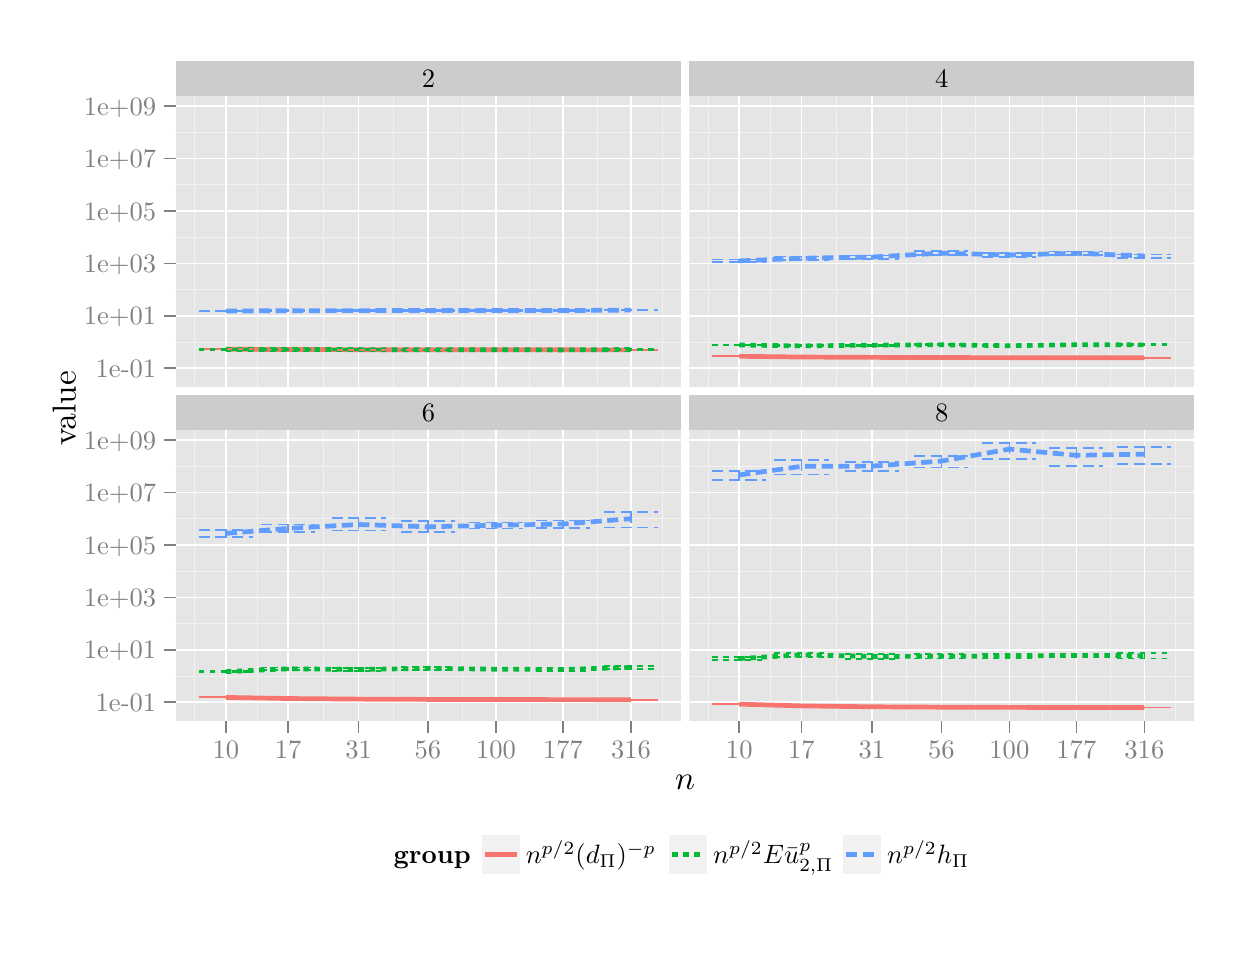
\begin{tikzpicture}[x=1pt,y=1pt]
\definecolor[named]{fillColor}{rgb}{1.00,1.00,1.00}
\path[use as bounding box,fill=fillColor,fill opacity=0.00] (0,0) rectangle (433.62,325.21);
\begin{scope}
\path[clip] (  0.00,  0.00) rectangle (433.62,325.21);
\definecolor[named]{drawColor}{rgb}{1.00,1.00,1.00}
\definecolor[named]{fillColor}{rgb}{1.00,1.00,1.00}

\path[draw=drawColor,line width= 0.6pt,line join=round,line cap=round,fill=fillColor] (  0.00,  0.00) rectangle (433.62,325.21);
\end{scope}
\begin{scope}
\path[clip] ( 53.55,195.47) rectangle (236.06,300.54);
\definecolor[named]{fillColor}{rgb}{0.90,0.90,0.90}

\path[fill=fillColor] ( 53.55,195.47) rectangle (236.06,300.54);
\definecolor[named]{drawColor}{rgb}{0.95,0.95,0.95}

\path[draw=drawColor,line width= 0.3pt,line join=round] ( 53.55,211.63) --
	(236.06,211.63);

\path[draw=drawColor,line width= 0.3pt,line join=round] ( 53.55,230.58) --
	(236.06,230.58);

\path[draw=drawColor,line width= 0.3pt,line join=round] ( 53.55,249.53) --
	(236.06,249.53);

\path[draw=drawColor,line width= 0.3pt,line join=round] ( 53.55,268.48) --
	(236.06,268.48);

\path[draw=drawColor,line width= 0.3pt,line join=round] ( 53.55,287.43) --
	(236.06,287.43);

\path[draw=drawColor,line width= 0.3pt,line join=round] ( 60.36,195.47) --
	( 60.36,300.54);

\path[draw=drawColor,line width= 0.3pt,line join=round] ( 82.85,195.47) --
	( 82.85,300.54);

\path[draw=drawColor,line width= 0.3pt,line join=round] (106.84,195.47) --
	(106.84,300.54);

\path[draw=drawColor,line width= 0.3pt,line join=round] (132.11,195.47) --
	(132.11,300.54);

\path[draw=drawColor,line width= 0.3pt,line join=round] (156.93,195.47) --
	(156.93,300.54);

\path[draw=drawColor,line width= 0.3pt,line join=round] (181.33,195.47) --
	(181.33,300.54);

\path[draw=drawColor,line width= 0.3pt,line join=round] (205.71,195.47) --
	(205.71,300.54);

\path[draw=drawColor,line width= 0.3pt,line join=round] (229.25,195.47) --
	(229.25,300.54);
\definecolor[named]{drawColor}{rgb}{1.00,1.00,1.00}

\path[draw=drawColor,line width= 0.6pt,line join=round] ( 53.55,202.15) --
	(236.06,202.15);

\path[draw=drawColor,line width= 0.6pt,line join=round] ( 53.55,221.10) --
	(236.06,221.10);

\path[draw=drawColor,line width= 0.6pt,line join=round] ( 53.55,240.05) --
	(236.06,240.05);

\path[draw=drawColor,line width= 0.6pt,line join=round] ( 53.55,259.00) --
	(236.06,259.00);

\path[draw=drawColor,line width= 0.6pt,line join=round] ( 53.55,277.95) --
	(236.06,277.95);

\path[draw=drawColor,line width= 0.6pt,line join=round] ( 53.55,296.90) --
	(236.06,296.90);

\path[draw=drawColor,line width= 0.6pt,line join=round] ( 71.61,195.47) --
	( 71.61,300.54);

\path[draw=drawColor,line width= 0.6pt,line join=round] ( 94.10,195.47) --
	( 94.10,300.54);

\path[draw=drawColor,line width= 0.6pt,line join=round] (119.57,195.47) --
	(119.57,300.54);

\path[draw=drawColor,line width= 0.6pt,line join=round] (144.64,195.47) --
	(144.64,300.54);

\path[draw=drawColor,line width= 0.6pt,line join=round] (169.22,195.47) --
	(169.22,300.54);

\path[draw=drawColor,line width= 0.6pt,line join=round] (193.43,195.47) --
	(193.43,300.54);

\path[draw=drawColor,line width= 0.6pt,line join=round] (218.00,195.47) --
	(218.00,300.54);
\definecolor[named]{drawColor}{rgb}{0.97,0.46,0.43}

\path[draw=drawColor,line width= 1.7pt,line join=round] ( 71.61,209.02) --
	( 94.10,208.91) --
	(119.57,208.85) --
	(144.64,208.82) --
	(169.22,208.80) --
	(193.43,208.79) --
	(218.00,208.78);
\definecolor[named]{drawColor}{rgb}{0.00,0.73,0.22}

\path[draw=drawColor,line width= 1.7pt,dash pattern=on 2pt off 2pt ,line join=round] ( 71.61,208.92) --
	( 94.10,208.93) --
	(119.57,208.88) --
	(144.64,208.81) --
	(169.22,208.82) --
	(193.43,208.76) --
	(218.00,208.91);
\definecolor[named]{drawColor}{rgb}{0.38,0.61,1.00}

\path[draw=drawColor,line width= 1.7pt,dash pattern=on 4pt off 2pt ,line join=round] ( 71.61,222.80) --
	( 94.10,222.95) --
	(119.57,222.96) --
	(144.64,223.01) --
	(169.22,223.00) --
	(193.43,222.99) --
	(218.00,223.15);
\definecolor[named]{drawColor}{rgb}{0.97,0.46,0.43}

\path[draw=drawColor,line width= 0.6pt,line join=round] ( 61.85,209.03) --
	( 81.37,209.03);

\path[draw=drawColor,line width= 0.6pt,line join=round] ( 71.61,209.03) --
	( 71.61,209.02);

\path[draw=drawColor,line width= 0.6pt,line join=round] ( 61.85,209.02) --
	( 81.37,209.02);

\path[draw=drawColor,line width= 0.6pt,line join=round] ( 84.34,208.92) --
	(103.86,208.92);

\path[draw=drawColor,line width= 0.6pt,line join=round] ( 94.10,208.92) --
	( 94.10,208.91);

\path[draw=drawColor,line width= 0.6pt,line join=round] ( 84.34,208.91) --
	(103.86,208.91);

\path[draw=drawColor,line width= 0.6pt,line join=round] (109.81,208.85) --
	(129.33,208.85);

\path[draw=drawColor,line width= 0.6pt,line join=round] (119.57,208.85) --
	(119.57,208.85);

\path[draw=drawColor,line width= 0.6pt,line join=round] (109.81,208.85) --
	(129.33,208.85);

\path[draw=drawColor,line width= 0.6pt,line join=round] (134.88,208.82) --
	(154.40,208.82);

\path[draw=drawColor,line width= 0.6pt,line join=round] (144.64,208.82) --
	(144.64,208.81);

\path[draw=drawColor,line width= 0.6pt,line join=round] (134.88,208.81) --
	(154.40,208.81);

\path[draw=drawColor,line width= 0.6pt,line join=round] (159.46,208.80) --
	(178.98,208.80);

\path[draw=drawColor,line width= 0.6pt,line join=round] (169.22,208.80) --
	(169.22,208.80);

\path[draw=drawColor,line width= 0.6pt,line join=round] (159.46,208.80) --
	(178.98,208.80);

\path[draw=drawColor,line width= 0.6pt,line join=round] (183.67,208.79) --
	(203.19,208.79);

\path[draw=drawColor,line width= 0.6pt,line join=round] (193.43,208.79) --
	(193.43,208.79);

\path[draw=drawColor,line width= 0.6pt,line join=round] (183.67,208.79) --
	(203.19,208.79);

\path[draw=drawColor,line width= 0.6pt,line join=round] (208.24,208.78) --
	(227.76,208.78);

\path[draw=drawColor,line width= 0.6pt,line join=round] (218.00,208.78) --
	(218.00,208.78);

\path[draw=drawColor,line width= 0.6pt,line join=round] (208.24,208.78) --
	(227.76,208.78);
\definecolor[named]{drawColor}{rgb}{0.00,0.73,0.22}

\path[draw=drawColor,line width= 0.6pt,dash pattern=on 2pt off 2pt ,line join=round] ( 61.85,209.03) --
	( 81.37,209.03);

\path[draw=drawColor,line width= 0.6pt,dash pattern=on 2pt off 2pt ,line join=round] ( 71.61,209.03) --
	( 71.61,208.81);

\path[draw=drawColor,line width= 0.6pt,dash pattern=on 2pt off 2pt ,line join=round] ( 61.85,208.81) --
	( 81.37,208.81);

\path[draw=drawColor,line width= 0.6pt,dash pattern=on 2pt off 2pt ,line join=round] ( 84.34,209.05) --
	(103.86,209.05);

\path[draw=drawColor,line width= 0.6pt,dash pattern=on 2pt off 2pt ,line join=round] ( 94.10,209.05) --
	( 94.10,208.82);

\path[draw=drawColor,line width= 0.6pt,dash pattern=on 2pt off 2pt ,line join=round] ( 84.34,208.82) --
	(103.86,208.82);

\path[draw=drawColor,line width= 0.6pt,dash pattern=on 2pt off 2pt ,line join=round] (109.81,208.98) --
	(129.33,208.98);

\path[draw=drawColor,line width= 0.6pt,dash pattern=on 2pt off 2pt ,line join=round] (119.57,208.98) --
	(119.57,208.76);

\path[draw=drawColor,line width= 0.6pt,dash pattern=on 2pt off 2pt ,line join=round] (109.81,208.76) --
	(129.33,208.76);

\path[draw=drawColor,line width= 0.6pt,dash pattern=on 2pt off 2pt ,line join=round] (134.88,208.91) --
	(154.40,208.91);

\path[draw=drawColor,line width= 0.6pt,dash pattern=on 2pt off 2pt ,line join=round] (144.64,208.91) --
	(144.64,208.69);

\path[draw=drawColor,line width= 0.6pt,dash pattern=on 2pt off 2pt ,line join=round] (134.88,208.69) --
	(154.40,208.69);

\path[draw=drawColor,line width= 0.6pt,dash pattern=on 2pt off 2pt ,line join=round] (159.46,208.94) --
	(178.98,208.94);

\path[draw=drawColor,line width= 0.6pt,dash pattern=on 2pt off 2pt ,line join=round] (169.22,208.94) --
	(169.22,208.71);

\path[draw=drawColor,line width= 0.6pt,dash pattern=on 2pt off 2pt ,line join=round] (159.46,208.71) --
	(178.98,208.71);

\path[draw=drawColor,line width= 0.6pt,dash pattern=on 2pt off 2pt ,line join=round] (183.67,208.88) --
	(203.19,208.88);

\path[draw=drawColor,line width= 0.6pt,dash pattern=on 2pt off 2pt ,line join=round] (193.43,208.88) --
	(193.43,208.65);

\path[draw=drawColor,line width= 0.6pt,dash pattern=on 2pt off 2pt ,line join=round] (183.67,208.65) --
	(203.19,208.65);

\path[draw=drawColor,line width= 0.6pt,dash pattern=on 2pt off 2pt ,line join=round] (208.24,209.01) --
	(227.76,209.01);

\path[draw=drawColor,line width= 0.6pt,dash pattern=on 2pt off 2pt ,line join=round] (218.00,209.01) --
	(218.00,208.80);

\path[draw=drawColor,line width= 0.6pt,dash pattern=on 2pt off 2pt ,line join=round] (208.24,208.80) --
	(227.76,208.80);
\definecolor[named]{drawColor}{rgb}{0.38,0.61,1.00}

\path[draw=drawColor,line width= 0.6pt,dash pattern=on 4pt off 2pt ,line join=round] ( 61.85,222.99) --
	( 81.37,222.99);

\path[draw=drawColor,line width= 0.6pt,dash pattern=on 4pt off 2pt ,line join=round] ( 71.61,222.99) --
	( 71.61,222.62);

\path[draw=drawColor,line width= 0.6pt,dash pattern=on 4pt off 2pt ,line join=round] ( 61.85,222.62) --
	( 81.37,222.62);

\path[draw=drawColor,line width= 0.6pt,dash pattern=on 4pt off 2pt ,line join=round] ( 84.34,223.13) --
	(103.86,223.13);

\path[draw=drawColor,line width= 0.6pt,dash pattern=on 4pt off 2pt ,line join=round] ( 94.10,223.13) --
	( 94.10,222.72);

\path[draw=drawColor,line width= 0.6pt,dash pattern=on 4pt off 2pt ,line join=round] ( 84.34,222.72) --
	(103.86,222.72);

\path[draw=drawColor,line width= 0.6pt,dash pattern=on 4pt off 2pt ,line join=round] (109.81,223.18) --
	(129.33,223.18);

\path[draw=drawColor,line width= 0.6pt,dash pattern=on 4pt off 2pt ,line join=round] (119.57,223.18) --
	(119.57,222.75);

\path[draw=drawColor,line width= 0.6pt,dash pattern=on 4pt off 2pt ,line join=round] (109.81,222.75) --
	(129.33,222.75);

\path[draw=drawColor,line width= 0.6pt,dash pattern=on 4pt off 2pt ,line join=round] (134.88,223.24) --
	(154.40,223.24);

\path[draw=drawColor,line width= 0.6pt,dash pattern=on 4pt off 2pt ,line join=round] (144.64,223.24) --
	(144.64,222.79);

\path[draw=drawColor,line width= 0.6pt,dash pattern=on 4pt off 2pt ,line join=round] (134.88,222.79) --
	(154.40,222.79);

\path[draw=drawColor,line width= 0.6pt,dash pattern=on 4pt off 2pt ,line join=round] (159.46,223.20) --
	(178.98,223.20);

\path[draw=drawColor,line width= 0.6pt,dash pattern=on 4pt off 2pt ,line join=round] (169.22,223.20) --
	(169.22,222.78);

\path[draw=drawColor,line width= 0.6pt,dash pattern=on 4pt off 2pt ,line join=round] (159.46,222.78) --
	(178.98,222.78);

\path[draw=drawColor,line width= 0.6pt,dash pattern=on 4pt off 2pt ,line join=round] (183.67,223.20) --
	(203.19,223.20);

\path[draw=drawColor,line width= 0.6pt,dash pattern=on 4pt off 2pt ,line join=round] (193.43,223.20) --
	(193.43,222.77);

\path[draw=drawColor,line width= 0.6pt,dash pattern=on 4pt off 2pt ,line join=round] (183.67,222.77) --
	(203.19,222.77);

\path[draw=drawColor,line width= 0.6pt,dash pattern=on 4pt off 2pt ,line join=round] (208.24,223.35) --
	(227.76,223.35);

\path[draw=drawColor,line width= 0.6pt,dash pattern=on 4pt off 2pt ,line join=round] (218.00,223.35) --
	(218.00,222.95);

\path[draw=drawColor,line width= 0.6pt,dash pattern=on 4pt off 2pt ,line join=round] (208.24,222.95) --
	(227.76,222.95);
\end{scope}
\begin{scope}
\path[clip] (239.07,195.47) rectangle (421.58,300.54);
\definecolor[named]{fillColor}{rgb}{0.90,0.90,0.90}

\path[fill=fillColor] (239.07,195.47) rectangle (421.57,300.54);
\definecolor[named]{drawColor}{rgb}{0.95,0.95,0.95}

\path[draw=drawColor,line width= 0.3pt,line join=round] (239.07,211.63) --
	(421.58,211.63);

\path[draw=drawColor,line width= 0.3pt,line join=round] (239.07,230.58) --
	(421.58,230.58);

\path[draw=drawColor,line width= 0.3pt,line join=round] (239.07,249.53) --
	(421.58,249.53);

\path[draw=drawColor,line width= 0.3pt,line join=round] (239.07,268.48) --
	(421.58,268.48);

\path[draw=drawColor,line width= 0.3pt,line join=round] (239.07,287.43) --
	(421.58,287.43);

\path[draw=drawColor,line width= 0.3pt,line join=round] (245.88,195.47) --
	(245.88,300.54);

\path[draw=drawColor,line width= 0.3pt,line join=round] (268.37,195.47) --
	(268.37,300.54);

\path[draw=drawColor,line width= 0.3pt,line join=round] (292.36,195.47) --
	(292.36,300.54);

\path[draw=drawColor,line width= 0.3pt,line join=round] (317.62,195.47) --
	(317.62,300.54);

\path[draw=drawColor,line width= 0.3pt,line join=round] (342.45,195.47) --
	(342.45,300.54);

\path[draw=drawColor,line width= 0.3pt,line join=round] (366.84,195.47) --
	(366.84,300.54);

\path[draw=drawColor,line width= 0.3pt,line join=round] (391.23,195.47) --
	(391.23,300.54);

\path[draw=drawColor,line width= 0.3pt,line join=round] (414.77,195.47) --
	(414.77,300.54);
\definecolor[named]{drawColor}{rgb}{1.00,1.00,1.00}

\path[draw=drawColor,line width= 0.6pt,line join=round] (239.07,202.15) --
	(421.58,202.15);

\path[draw=drawColor,line width= 0.6pt,line join=round] (239.07,221.10) --
	(421.58,221.10);

\path[draw=drawColor,line width= 0.6pt,line join=round] (239.07,240.05) --
	(421.58,240.05);

\path[draw=drawColor,line width= 0.6pt,line join=round] (239.07,259.00) --
	(421.58,259.00);

\path[draw=drawColor,line width= 0.6pt,line join=round] (239.07,277.95) --
	(421.58,277.95);

\path[draw=drawColor,line width= 0.6pt,line join=round] (239.07,296.90) --
	(421.58,296.90);

\path[draw=drawColor,line width= 0.6pt,line join=round] (257.13,195.47) --
	(257.13,300.54);

\path[draw=drawColor,line width= 0.6pt,line join=round] (279.62,195.47) --
	(279.62,300.54);

\path[draw=drawColor,line width= 0.6pt,line join=round] (305.09,195.47) --
	(305.09,300.54);

\path[draw=drawColor,line width= 0.6pt,line join=round] (330.16,195.47) --
	(330.16,300.54);

\path[draw=drawColor,line width= 0.6pt,line join=round] (354.74,195.47) --
	(354.74,300.54);

\path[draw=drawColor,line width= 0.6pt,line join=round] (378.95,195.47) --
	(378.95,300.54);

\path[draw=drawColor,line width= 0.6pt,line join=round] (403.52,195.47) --
	(403.52,300.54);
\definecolor[named]{drawColor}{rgb}{0.97,0.46,0.43}

\path[draw=drawColor,line width= 1.7pt,line join=round] (257.13,206.46) --
	(279.62,206.19) --
	(305.09,206.07) --
	(330.16,206.00) --
	(354.74,205.97) --
	(378.95,205.95) --
	(403.52,205.94);
\definecolor[named]{drawColor}{rgb}{0.00,0.73,0.22}

\path[draw=drawColor,line width= 1.7pt,dash pattern=on 2pt off 2pt ,line join=round] (257.13,210.53) --
	(279.62,210.21) --
	(305.09,210.48) --
	(330.16,210.61) --
	(354.74,210.28) --
	(378.95,210.65) --
	(403.52,210.58);
\definecolor[named]{drawColor}{rgb}{0.38,0.61,1.00}

\path[draw=drawColor,line width= 1.7pt,dash pattern=on 4pt off 2pt ,line join=round] (257.13,240.93) --
	(279.62,241.89) --
	(305.09,242.33) --
	(330.16,243.73) --
	(354.74,243.07) --
	(378.95,243.68) --
	(403.52,242.72);
\definecolor[named]{drawColor}{rgb}{0.97,0.46,0.43}

\path[draw=drawColor,line width= 0.6pt,line join=round] (247.36,206.48) --
	(266.89,206.48);

\path[draw=drawColor,line width= 0.6pt,line join=round] (257.13,206.48) --
	(257.13,206.44);

\path[draw=drawColor,line width= 0.6pt,line join=round] (247.36,206.44) --
	(266.89,206.44);

\path[draw=drawColor,line width= 0.6pt,line join=round] (269.86,206.20) --
	(289.38,206.20);

\path[draw=drawColor,line width= 0.6pt,line join=round] (279.62,206.20) --
	(279.62,206.19);

\path[draw=drawColor,line width= 0.6pt,line join=round] (269.86,206.19) --
	(289.38,206.19);

\path[draw=drawColor,line width= 0.6pt,line join=round] (295.33,206.07) --
	(314.85,206.07);

\path[draw=drawColor,line width= 0.6pt,line join=round] (305.09,206.07) --
	(305.09,206.06);

\path[draw=drawColor,line width= 0.6pt,line join=round] (295.33,206.06) --
	(314.85,206.06);

\path[draw=drawColor,line width= 0.6pt,line join=round] (320.40,206.00) --
	(339.92,206.00);

\path[draw=drawColor,line width= 0.6pt,line join=round] (330.16,206.00) --
	(330.16,206.00);

\path[draw=drawColor,line width= 0.6pt,line join=round] (320.40,206.00) --
	(339.92,206.00);

\path[draw=drawColor,line width= 0.6pt,line join=round] (344.98,205.97) --
	(364.50,205.97);

\path[draw=drawColor,line width= 0.6pt,line join=round] (354.74,205.97) --
	(354.74,205.97);

\path[draw=drawColor,line width= 0.6pt,line join=round] (344.98,205.97) --
	(364.50,205.97);

\path[draw=drawColor,line width= 0.6pt,line join=round] (369.19,205.95) --
	(388.71,205.95);

\path[draw=drawColor,line width= 0.6pt,line join=round] (378.95,205.95) --
	(378.95,205.95);

\path[draw=drawColor,line width= 0.6pt,line join=round] (369.19,205.95) --
	(388.71,205.95);

\path[draw=drawColor,line width= 0.6pt,line join=round] (393.76,205.94) --
	(413.28,205.94);

\path[draw=drawColor,line width= 0.6pt,line join=round] (403.52,205.94) --
	(403.52,205.94);

\path[draw=drawColor,line width= 0.6pt,line join=round] (393.76,205.94) --
	(413.28,205.94);
\definecolor[named]{drawColor}{rgb}{0.00,0.73,0.22}

\path[draw=drawColor,line width= 0.6pt,dash pattern=on 2pt off 2pt ,line join=round] (247.36,210.75) --
	(266.89,210.75);

\path[draw=drawColor,line width= 0.6pt,dash pattern=on 2pt off 2pt ,line join=round] (257.13,210.75) --
	(257.13,210.31);

\path[draw=drawColor,line width= 0.6pt,dash pattern=on 2pt off 2pt ,line join=round] (247.36,210.31) --
	(266.89,210.31);

\path[draw=drawColor,line width= 0.6pt,dash pattern=on 2pt off 2pt ,line join=round] (269.86,210.44) --
	(289.38,210.44);

\path[draw=drawColor,line width= 0.6pt,dash pattern=on 2pt off 2pt ,line join=round] (279.62,210.44) --
	(279.62,209.97);

\path[draw=drawColor,line width= 0.6pt,dash pattern=on 2pt off 2pt ,line join=round] (269.86,209.97) --
	(289.38,209.97);

\path[draw=drawColor,line width= 0.6pt,dash pattern=on 2pt off 2pt ,line join=round] (295.33,210.74) --
	(314.85,210.74);

\path[draw=drawColor,line width= 0.6pt,dash pattern=on 2pt off 2pt ,line join=round] (305.09,210.74) --
	(305.09,210.22);

\path[draw=drawColor,line width= 0.6pt,dash pattern=on 2pt off 2pt ,line join=round] (295.33,210.22) --
	(314.85,210.22);

\path[draw=drawColor,line width= 0.6pt,dash pattern=on 2pt off 2pt ,line join=round] (320.40,210.88) --
	(339.92,210.88);

\path[draw=drawColor,line width= 0.6pt,dash pattern=on 2pt off 2pt ,line join=round] (330.16,210.88) --
	(330.16,210.33);

\path[draw=drawColor,line width= 0.6pt,dash pattern=on 2pt off 2pt ,line join=round] (320.40,210.33) --
	(339.92,210.33);

\path[draw=drawColor,line width= 0.6pt,dash pattern=on 2pt off 2pt ,line join=round] (344.98,210.54) --
	(364.50,210.54);

\path[draw=drawColor,line width= 0.6pt,dash pattern=on 2pt off 2pt ,line join=round] (354.74,210.54) --
	(354.74,210.02);

\path[draw=drawColor,line width= 0.6pt,dash pattern=on 2pt off 2pt ,line join=round] (344.98,210.02) --
	(364.50,210.02);

\path[draw=drawColor,line width= 0.6pt,dash pattern=on 2pt off 2pt ,line join=round] (369.19,210.90) --
	(388.71,210.90);

\path[draw=drawColor,line width= 0.6pt,dash pattern=on 2pt off 2pt ,line join=round] (378.95,210.90) --
	(378.95,210.35);

\path[draw=drawColor,line width= 0.6pt,dash pattern=on 2pt off 2pt ,line join=round] (369.19,210.35) --
	(388.71,210.35);

\path[draw=drawColor,line width= 0.6pt,dash pattern=on 2pt off 2pt ,line join=round] (393.76,210.83) --
	(413.28,210.83);

\path[draw=drawColor,line width= 0.6pt,dash pattern=on 2pt off 2pt ,line join=round] (403.52,210.83) --
	(403.52,210.32);

\path[draw=drawColor,line width= 0.6pt,dash pattern=on 2pt off 2pt ,line join=round] (393.76,210.32) --
	(413.28,210.32);
\definecolor[named]{drawColor}{rgb}{0.38,0.61,1.00}

\path[draw=drawColor,line width= 0.6pt,dash pattern=on 4pt off 2pt ,line join=round] (247.36,241.41) --
	(266.89,241.41);

\path[draw=drawColor,line width= 0.6pt,dash pattern=on 4pt off 2pt ,line join=round] (257.13,241.41) --
	(257.13,240.45);

\path[draw=drawColor,line width= 0.6pt,dash pattern=on 4pt off 2pt ,line join=round] (247.36,240.45) --
	(266.89,240.45);

\path[draw=drawColor,line width= 0.6pt,dash pattern=on 4pt off 2pt ,line join=round] (269.86,242.52) --
	(289.38,242.52);

\path[draw=drawColor,line width= 0.6pt,dash pattern=on 4pt off 2pt ,line join=round] (279.62,242.52) --
	(279.62,241.30);

\path[draw=drawColor,line width= 0.6pt,dash pattern=on 4pt off 2pt ,line join=round] (269.86,241.30) --
	(289.38,241.30);

\path[draw=drawColor,line width= 0.6pt,dash pattern=on 4pt off 2pt ,line join=round] (295.33,242.91) --
	(314.85,242.91);

\path[draw=drawColor,line width= 0.6pt,dash pattern=on 4pt off 2pt ,line join=round] (305.09,242.91) --
	(305.09,241.71);

\path[draw=drawColor,line width= 0.6pt,dash pattern=on 4pt off 2pt ,line join=round] (295.33,241.71) --
	(314.85,241.71);

\path[draw=drawColor,line width= 0.6pt,dash pattern=on 4pt off 2pt ,line join=round] (320.40,244.46) --
	(339.92,244.46);

\path[draw=drawColor,line width= 0.6pt,dash pattern=on 4pt off 2pt ,line join=round] (330.16,244.46) --
	(330.16,243.02);

\path[draw=drawColor,line width= 0.6pt,dash pattern=on 4pt off 2pt ,line join=round] (320.40,243.02) --
	(339.92,243.02);

\path[draw=drawColor,line width= 0.6pt,dash pattern=on 4pt off 2pt ,line join=round] (344.98,243.67) --
	(364.50,243.67);

\path[draw=drawColor,line width= 0.6pt,dash pattern=on 4pt off 2pt ,line join=round] (354.74,243.67) --
	(354.74,242.36);

\path[draw=drawColor,line width= 0.6pt,dash pattern=on 4pt off 2pt ,line join=round] (344.98,242.36) --
	(364.50,242.36);

\path[draw=drawColor,line width= 0.6pt,dash pattern=on 4pt off 2pt ,line join=round] (369.19,244.32) --
	(388.71,244.32);

\path[draw=drawColor,line width= 0.6pt,dash pattern=on 4pt off 2pt ,line join=round] (378.95,244.32) --
	(378.95,243.05);

\path[draw=drawColor,line width= 0.6pt,dash pattern=on 4pt off 2pt ,line join=round] (369.19,243.05) --
	(388.71,243.05);

\path[draw=drawColor,line width= 0.6pt,dash pattern=on 4pt off 2pt ,line join=round] (393.76,243.28) --
	(413.28,243.28);

\path[draw=drawColor,line width= 0.6pt,dash pattern=on 4pt off 2pt ,line join=round] (403.52,243.28) --
	(403.52,242.09);

\path[draw=drawColor,line width= 0.6pt,dash pattern=on 4pt off 2pt ,line join=round] (393.76,242.09) --
	(413.28,242.09);
\end{scope}
\begin{scope}
\path[clip] ( 53.55, 74.76) rectangle (236.06,179.83);
\definecolor[named]{fillColor}{rgb}{0.90,0.90,0.90}

\path[fill=fillColor] ( 53.55, 74.76) rectangle (236.06,179.83);
\definecolor[named]{drawColor}{rgb}{0.95,0.95,0.95}

\path[draw=drawColor,line width= 0.3pt,line join=round] ( 53.55, 90.92) --
	(236.06, 90.92);

\path[draw=drawColor,line width= 0.3pt,line join=round] ( 53.55,109.87) --
	(236.06,109.87);

\path[draw=drawColor,line width= 0.3pt,line join=round] ( 53.55,128.82) --
	(236.06,128.82);

\path[draw=drawColor,line width= 0.3pt,line join=round] ( 53.55,147.77) --
	(236.06,147.77);

\path[draw=drawColor,line width= 0.3pt,line join=round] ( 53.55,166.72) --
	(236.06,166.72);

\path[draw=drawColor,line width= 0.3pt,line join=round] ( 60.36, 74.76) --
	( 60.36,179.83);

\path[draw=drawColor,line width= 0.3pt,line join=round] ( 82.85, 74.76) --
	( 82.85,179.83);

\path[draw=drawColor,line width= 0.3pt,line join=round] (106.84, 74.76) --
	(106.84,179.83);

\path[draw=drawColor,line width= 0.3pt,line join=round] (132.11, 74.76) --
	(132.11,179.83);

\path[draw=drawColor,line width= 0.3pt,line join=round] (156.93, 74.76) --
	(156.93,179.83);

\path[draw=drawColor,line width= 0.3pt,line join=round] (181.33, 74.76) --
	(181.33,179.83);

\path[draw=drawColor,line width= 0.3pt,line join=round] (205.71, 74.76) --
	(205.71,179.83);

\path[draw=drawColor,line width= 0.3pt,line join=round] (229.25, 74.76) --
	(229.25,179.83);
\definecolor[named]{drawColor}{rgb}{1.00,1.00,1.00}

\path[draw=drawColor,line width= 0.6pt,line join=round] ( 53.55, 81.44) --
	(236.06, 81.44);

\path[draw=drawColor,line width= 0.6pt,line join=round] ( 53.55,100.39) --
	(236.06,100.39);

\path[draw=drawColor,line width= 0.6pt,line join=round] ( 53.55,119.34) --
	(236.06,119.34);

\path[draw=drawColor,line width= 0.6pt,line join=round] ( 53.55,138.29) --
	(236.06,138.29);

\path[draw=drawColor,line width= 0.6pt,line join=round] ( 53.55,157.24) --
	(236.06,157.24);

\path[draw=drawColor,line width= 0.6pt,line join=round] ( 53.55,176.19) --
	(236.06,176.19);

\path[draw=drawColor,line width= 0.6pt,line join=round] ( 71.61, 74.76) --
	( 71.61,179.83);

\path[draw=drawColor,line width= 0.6pt,line join=round] ( 94.10, 74.76) --
	( 94.10,179.83);

\path[draw=drawColor,line width= 0.6pt,line join=round] (119.57, 74.76) --
	(119.57,179.83);

\path[draw=drawColor,line width= 0.6pt,line join=round] (144.64, 74.76) --
	(144.64,179.83);

\path[draw=drawColor,line width= 0.6pt,line join=round] (169.22, 74.76) --
	(169.22,179.83);

\path[draw=drawColor,line width= 0.6pt,line join=round] (193.43, 74.76) --
	(193.43,179.83);

\path[draw=drawColor,line width= 0.6pt,line join=round] (218.00, 74.76) --
	(218.00,179.83);
\definecolor[named]{drawColor}{rgb}{0.97,0.46,0.43}

\path[draw=drawColor,line width= 1.7pt,line join=round] ( 71.61, 83.20) --
	( 94.10, 82.80) --
	(119.57, 82.58) --
	(144.64, 82.48) --
	(169.22, 82.43) --
	(193.43, 82.40) --
	(218.00, 82.38);
\definecolor[named]{drawColor}{rgb}{0.00,0.73,0.22}

\path[draw=drawColor,line width= 1.7pt,dash pattern=on 2pt off 2pt ,line join=round] ( 71.61, 92.51) --
	( 94.10, 93.54) --
	(119.57, 93.27) --
	(144.64, 93.71) --
	(169.22, 93.39) --
	(193.43, 93.30) --
	(218.00, 94.02);
\definecolor[named]{drawColor}{rgb}{0.38,0.61,1.00}

\path[draw=drawColor,line width= 1.7pt,dash pattern=on 4pt off 2pt ,line join=round] ( 71.61,142.46) --
	( 94.10,144.28) --
	(119.57,145.68) --
	(144.64,144.85) --
	(169.22,145.41) --
	(193.43,145.85) --
	(218.00,147.78);
\definecolor[named]{drawColor}{rgb}{0.97,0.46,0.43}

\path[draw=drawColor,line width= 0.6pt,line join=round] ( 61.85, 83.23) --
	( 81.37, 83.23);

\path[draw=drawColor,line width= 0.6pt,line join=round] ( 71.61, 83.23) --
	( 71.61, 83.17);

\path[draw=drawColor,line width= 0.6pt,line join=round] ( 61.85, 83.17) --
	( 81.37, 83.17);

\path[draw=drawColor,line width= 0.6pt,line join=round] ( 84.34, 82.81) --
	(103.86, 82.81);

\path[draw=drawColor,line width= 0.6pt,line join=round] ( 94.10, 82.81) --
	( 94.10, 82.79);

\path[draw=drawColor,line width= 0.6pt,line join=round] ( 84.34, 82.79) --
	(103.86, 82.79);

\path[draw=drawColor,line width= 0.6pt,line join=round] (109.81, 82.59) --
	(129.33, 82.59);

\path[draw=drawColor,line width= 0.6pt,line join=round] (119.57, 82.59) --
	(119.57, 82.57);

\path[draw=drawColor,line width= 0.6pt,line join=round] (109.81, 82.57) --
	(129.33, 82.57);

\path[draw=drawColor,line width= 0.6pt,line join=round] (134.88, 82.48) --
	(154.40, 82.48);

\path[draw=drawColor,line width= 0.6pt,line join=round] (144.64, 82.48) --
	(144.64, 82.48);

\path[draw=drawColor,line width= 0.6pt,line join=round] (134.88, 82.48) --
	(154.40, 82.48);

\path[draw=drawColor,line width= 0.6pt,line join=round] (159.46, 82.43) --
	(178.98, 82.43);

\path[draw=drawColor,line width= 0.6pt,line join=round] (169.22, 82.43) --
	(169.22, 82.42);

\path[draw=drawColor,line width= 0.6pt,line join=round] (159.46, 82.42) --
	(178.98, 82.42);

\path[draw=drawColor,line width= 0.6pt,line join=round] (183.67, 82.40) --
	(203.19, 82.40);

\path[draw=drawColor,line width= 0.6pt,line join=round] (193.43, 82.40) --
	(193.43, 82.40);

\path[draw=drawColor,line width= 0.6pt,line join=round] (183.67, 82.40) --
	(203.19, 82.40);

\path[draw=drawColor,line width= 0.6pt,line join=round] (208.24, 82.38) --
	(227.76, 82.38);

\path[draw=drawColor,line width= 0.6pt,line join=round] (218.00, 82.38) --
	(218.00, 82.38);

\path[draw=drawColor,line width= 0.6pt,line join=round] (208.24, 82.38) --
	(227.76, 82.38);
\definecolor[named]{drawColor}{rgb}{0.00,0.73,0.22}

\path[draw=drawColor,line width= 0.6pt,dash pattern=on 2pt off 2pt ,line join=round] ( 61.85, 92.83) --
	( 81.37, 92.83);

\path[draw=drawColor,line width= 0.6pt,dash pattern=on 2pt off 2pt ,line join=round] ( 71.61, 92.83) --
	( 71.61, 92.20);

\path[draw=drawColor,line width= 0.6pt,dash pattern=on 2pt off 2pt ,line join=round] ( 61.85, 92.20) --
	( 81.37, 92.20);

\path[draw=drawColor,line width= 0.6pt,dash pattern=on 2pt off 2pt ,line join=round] ( 84.34, 94.01) --
	(103.86, 94.01);

\path[draw=drawColor,line width= 0.6pt,dash pattern=on 2pt off 2pt ,line join=round] ( 94.10, 94.01) --
	( 94.10, 93.07);

\path[draw=drawColor,line width= 0.6pt,dash pattern=on 2pt off 2pt ,line join=round] ( 84.34, 93.07) --
	(103.86, 93.07);

\path[draw=drawColor,line width= 0.6pt,dash pattern=on 2pt off 2pt ,line join=round] (109.81, 93.73) --
	(129.33, 93.73);

\path[draw=drawColor,line width= 0.6pt,dash pattern=on 2pt off 2pt ,line join=round] (119.57, 93.73) --
	(119.57, 92.82);

\path[draw=drawColor,line width= 0.6pt,dash pattern=on 2pt off 2pt ,line join=round] (109.81, 92.82) --
	(129.33, 92.82);

\path[draw=drawColor,line width= 0.6pt,dash pattern=on 2pt off 2pt ,line join=round] (134.88, 94.26) --
	(154.40, 94.26);

\path[draw=drawColor,line width= 0.6pt,dash pattern=on 2pt off 2pt ,line join=round] (144.64, 94.26) --
	(144.64, 93.11);

\path[draw=drawColor,line width= 0.6pt,dash pattern=on 2pt off 2pt ,line join=round] (134.88, 93.11) --
	(154.40, 93.11);

\path[draw=drawColor,line width= 0.6pt,dash pattern=on 2pt off 2pt ,line join=round] (159.46, 93.84) --
	(178.98, 93.84);

\path[draw=drawColor,line width= 0.6pt,dash pattern=on 2pt off 2pt ,line join=round] (169.22, 93.84) --
	(169.22, 92.89);

\path[draw=drawColor,line width= 0.6pt,dash pattern=on 2pt off 2pt ,line join=round] (159.46, 92.89) --
	(178.98, 92.89);

\path[draw=drawColor,line width= 0.6pt,dash pattern=on 2pt off 2pt ,line join=round] (183.67, 93.85) --
	(203.19, 93.85);

\path[draw=drawColor,line width= 0.6pt,dash pattern=on 2pt off 2pt ,line join=round] (193.43, 93.85) --
	(193.43, 92.78);

\path[draw=drawColor,line width= 0.6pt,dash pattern=on 2pt off 2pt ,line join=round] (183.67, 92.78) --
	(203.19, 92.78);

\path[draw=drawColor,line width= 0.6pt,dash pattern=on 2pt off 2pt ,line join=round] (208.24, 94.56) --
	(227.76, 94.56);

\path[draw=drawColor,line width= 0.6pt,dash pattern=on 2pt off 2pt ,line join=round] (218.00, 94.56) --
	(218.00, 93.47);

\path[draw=drawColor,line width= 0.6pt,dash pattern=on 2pt off 2pt ,line join=round] (208.24, 93.47) --
	(227.76, 93.47);
\definecolor[named]{drawColor}{rgb}{0.38,0.61,1.00}

\path[draw=drawColor,line width= 0.6pt,dash pattern=on 4pt off 2pt ,line join=round] ( 61.85,143.71) --
	( 81.37,143.71);

\path[draw=drawColor,line width= 0.6pt,dash pattern=on 4pt off 2pt ,line join=round] ( 71.61,143.71) --
	( 71.61,141.17);

\path[draw=drawColor,line width= 0.6pt,dash pattern=on 4pt off 2pt ,line join=round] ( 61.85,141.17) --
	( 81.37,141.17);

\path[draw=drawColor,line width= 0.6pt,dash pattern=on 4pt off 2pt ,line join=round] ( 84.34,145.62) --
	(103.86,145.62);

\path[draw=drawColor,line width= 0.6pt,dash pattern=on 4pt off 2pt ,line join=round] ( 94.10,145.62) --
	( 94.10,142.94);

\path[draw=drawColor,line width= 0.6pt,dash pattern=on 4pt off 2pt ,line join=round] ( 84.34,142.94) --
	(103.86,142.94);

\path[draw=drawColor,line width= 0.6pt,dash pattern=on 4pt off 2pt ,line join=round] (109.81,147.97) --
	(129.33,147.97);

\path[draw=drawColor,line width= 0.6pt,dash pattern=on 4pt off 2pt ,line join=round] (119.57,147.97) --
	(119.57,143.48);

\path[draw=drawColor,line width= 0.6pt,dash pattern=on 4pt off 2pt ,line join=round] (109.81,143.48) --
	(129.33,143.48);

\path[draw=drawColor,line width= 0.6pt,dash pattern=on 4pt off 2pt ,line join=round] (134.88,146.91) --
	(154.40,146.91);

\path[draw=drawColor,line width= 0.6pt,dash pattern=on 4pt off 2pt ,line join=round] (144.64,146.91) --
	(144.64,142.91);

\path[draw=drawColor,line width= 0.6pt,dash pattern=on 4pt off 2pt ,line join=round] (134.88,142.91) --
	(154.40,142.91);

\path[draw=drawColor,line width= 0.6pt,dash pattern=on 4pt off 2pt ,line join=round] (159.46,146.36) --
	(178.98,146.36);

\path[draw=drawColor,line width= 0.6pt,dash pattern=on 4pt off 2pt ,line join=round] (169.22,146.36) --
	(169.22,144.23);

\path[draw=drawColor,line width= 0.6pt,dash pattern=on 4pt off 2pt ,line join=round] (159.46,144.23) --
	(178.98,144.23);

\path[draw=drawColor,line width= 0.6pt,dash pattern=on 4pt off 2pt ,line join=round] (183.67,147.17) --
	(203.19,147.17);

\path[draw=drawColor,line width= 0.6pt,dash pattern=on 4pt off 2pt ,line join=round] (193.43,147.17) --
	(193.43,144.41);

\path[draw=drawColor,line width= 0.6pt,dash pattern=on 4pt off 2pt ,line join=round] (183.67,144.41) --
	(203.19,144.41);

\path[draw=drawColor,line width= 0.6pt,dash pattern=on 4pt off 2pt ,line join=round] (208.24,150.26) --
	(227.76,150.26);

\path[draw=drawColor,line width= 0.6pt,dash pattern=on 4pt off 2pt ,line join=round] (218.00,150.26) --
	(218.00,144.60);

\path[draw=drawColor,line width= 0.6pt,dash pattern=on 4pt off 2pt ,line join=round] (208.24,144.60) --
	(227.76,144.60);
\end{scope}
\begin{scope}
\path[clip] (239.07, 74.76) rectangle (421.58,179.83);
\definecolor[named]{fillColor}{rgb}{0.90,0.90,0.90}

\path[fill=fillColor] (239.07, 74.76) rectangle (421.57,179.83);
\definecolor[named]{drawColor}{rgb}{0.95,0.95,0.95}

\path[draw=drawColor,line width= 0.3pt,line join=round] (239.07, 90.92) --
	(421.58, 90.92);

\path[draw=drawColor,line width= 0.3pt,line join=round] (239.07,109.87) --
	(421.58,109.87);

\path[draw=drawColor,line width= 0.3pt,line join=round] (239.07,128.82) --
	(421.58,128.82);

\path[draw=drawColor,line width= 0.3pt,line join=round] (239.07,147.77) --
	(421.58,147.77);

\path[draw=drawColor,line width= 0.3pt,line join=round] (239.07,166.72) --
	(421.58,166.72);

\path[draw=drawColor,line width= 0.3pt,line join=round] (245.88, 74.76) --
	(245.88,179.83);

\path[draw=drawColor,line width= 0.3pt,line join=round] (268.37, 74.76) --
	(268.37,179.83);

\path[draw=drawColor,line width= 0.3pt,line join=round] (292.36, 74.76) --
	(292.36,179.83);

\path[draw=drawColor,line width= 0.3pt,line join=round] (317.62, 74.76) --
	(317.62,179.83);

\path[draw=drawColor,line width= 0.3pt,line join=round] (342.45, 74.76) --
	(342.45,179.83);

\path[draw=drawColor,line width= 0.3pt,line join=round] (366.84, 74.76) --
	(366.84,179.83);

\path[draw=drawColor,line width= 0.3pt,line join=round] (391.23, 74.76) --
	(391.23,179.83);

\path[draw=drawColor,line width= 0.3pt,line join=round] (414.77, 74.76) --
	(414.77,179.83);
\definecolor[named]{drawColor}{rgb}{1.00,1.00,1.00}

\path[draw=drawColor,line width= 0.6pt,line join=round] (239.07, 81.44) --
	(421.58, 81.44);

\path[draw=drawColor,line width= 0.6pt,line join=round] (239.07,100.39) --
	(421.58,100.39);

\path[draw=drawColor,line width= 0.6pt,line join=round] (239.07,119.34) --
	(421.58,119.34);

\path[draw=drawColor,line width= 0.6pt,line join=round] (239.07,138.29) --
	(421.58,138.29);

\path[draw=drawColor,line width= 0.6pt,line join=round] (239.07,157.24) --
	(421.58,157.24);

\path[draw=drawColor,line width= 0.6pt,line join=round] (239.07,176.19) --
	(421.58,176.19);

\path[draw=drawColor,line width= 0.6pt,line join=round] (257.13, 74.76) --
	(257.13,179.83);

\path[draw=drawColor,line width= 0.6pt,line join=round] (279.62, 74.76) --
	(279.62,179.83);

\path[draw=drawColor,line width= 0.6pt,line join=round] (305.09, 74.76) --
	(305.09,179.83);

\path[draw=drawColor,line width= 0.6pt,line join=round] (330.16, 74.76) --
	(330.16,179.83);

\path[draw=drawColor,line width= 0.6pt,line join=round] (354.74, 74.76) --
	(354.74,179.83);

\path[draw=drawColor,line width= 0.6pt,line join=round] (378.95, 74.76) --
	(378.95,179.83);

\path[draw=drawColor,line width= 0.6pt,line join=round] (403.52, 74.76) --
	(403.52,179.83);
\definecolor[named]{drawColor}{rgb}{0.97,0.46,0.43}

\path[draw=drawColor,line width= 1.7pt,line join=round] (257.13, 80.76) --
	(279.62, 80.13) --
	(305.09, 79.81) --
	(330.16, 79.67) --
	(354.74, 79.60) --
	(378.95, 79.56) --
	(403.52, 79.54);
\definecolor[named]{drawColor}{rgb}{0.00,0.73,0.22}

\path[draw=drawColor,line width= 1.7pt,dash pattern=on 2pt off 2pt ,line join=round] (257.13, 97.24) --
	(279.62, 98.58) --
	(305.09, 97.98) --
	(330.16, 98.07) --
	(354.74, 98.13) --
	(378.95, 98.39) --
	(403.52, 98.27);
\definecolor[named]{drawColor}{rgb}{0.38,0.61,1.00}

\path[draw=drawColor,line width= 1.7pt,dash pattern=on 4pt off 2pt ,line join=round] (257.13,163.58) --
	(279.62,166.69) --
	(305.09,166.78) --
	(330.16,168.59) --
	(354.74,172.92) --
	(378.95,170.67) --
	(403.52,171.10);
\definecolor[named]{drawColor}{rgb}{0.97,0.46,0.43}

\path[draw=drawColor,line width= 0.6pt,line join=round] (247.36, 80.82) --
	(266.89, 80.82);

\path[draw=drawColor,line width= 0.6pt,line join=round] (257.13, 80.82) --
	(257.13, 80.71);

\path[draw=drawColor,line width= 0.6pt,line join=round] (247.36, 80.71) --
	(266.89, 80.71);

\path[draw=drawColor,line width= 0.6pt,line join=round] (269.86, 80.15) --
	(289.38, 80.15);

\path[draw=drawColor,line width= 0.6pt,line join=round] (279.62, 80.15) --
	(279.62, 80.10);

\path[draw=drawColor,line width= 0.6pt,line join=round] (269.86, 80.10) --
	(289.38, 80.10);

\path[draw=drawColor,line width= 0.6pt,line join=round] (295.33, 79.82) --
	(314.85, 79.82);

\path[draw=drawColor,line width= 0.6pt,line join=round] (305.09, 79.82) --
	(305.09, 79.80);

\path[draw=drawColor,line width= 0.6pt,line join=round] (295.33, 79.80) --
	(314.85, 79.80);

\path[draw=drawColor,line width= 0.6pt,line join=round] (320.40, 79.67) --
	(339.92, 79.67);

\path[draw=drawColor,line width= 0.6pt,line join=round] (330.16, 79.67) --
	(330.16, 79.66);

\path[draw=drawColor,line width= 0.6pt,line join=round] (320.40, 79.66) --
	(339.92, 79.66);

\path[draw=drawColor,line width= 0.6pt,line join=round] (344.98, 79.60) --
	(364.50, 79.60);

\path[draw=drawColor,line width= 0.6pt,line join=round] (354.74, 79.60) --
	(354.74, 79.59);

\path[draw=drawColor,line width= 0.6pt,line join=round] (344.98, 79.59) --
	(364.50, 79.59);

\path[draw=drawColor,line width= 0.6pt,line join=round] (369.19, 79.56) --
	(388.71, 79.56);

\path[draw=drawColor,line width= 0.6pt,line join=round] (378.95, 79.56) --
	(378.95, 79.56);

\path[draw=drawColor,line width= 0.6pt,line join=round] (369.19, 79.56) --
	(388.71, 79.56);

\path[draw=drawColor,line width= 0.6pt,line join=round] (393.76, 79.54) --
	(413.28, 79.54);

\path[draw=drawColor,line width= 0.6pt,line join=round] (403.52, 79.54) --
	(403.52, 79.54);

\path[draw=drawColor,line width= 0.6pt,line join=round] (393.76, 79.54) --
	(413.28, 79.54);
\definecolor[named]{drawColor}{rgb}{0.00,0.73,0.22}

\path[draw=drawColor,line width= 0.6pt,dash pattern=on 2pt off 2pt ,line join=round] (247.36, 97.78) --
	(266.89, 97.78);

\path[draw=drawColor,line width= 0.6pt,dash pattern=on 2pt off 2pt ,line join=round] (257.13, 97.78) --
	(257.13, 96.71);

\path[draw=drawColor,line width= 0.6pt,dash pattern=on 2pt off 2pt ,line join=round] (247.36, 96.71) --
	(266.89, 96.71);

\path[draw=drawColor,line width= 0.6pt,dash pattern=on 2pt off 2pt ,line join=round] (269.86, 99.26) --
	(289.38, 99.26);

\path[draw=drawColor,line width= 0.6pt,dash pattern=on 2pt off 2pt ,line join=round] (279.62, 99.26) --
	(279.62, 97.77);

\path[draw=drawColor,line width= 0.6pt,dash pattern=on 2pt off 2pt ,line join=round] (269.86, 97.77) --
	(289.38, 97.77);

\path[draw=drawColor,line width= 0.6pt,dash pattern=on 2pt off 2pt ,line join=round] (295.33, 98.84) --
	(314.85, 98.84);

\path[draw=drawColor,line width= 0.6pt,dash pattern=on 2pt off 2pt ,line join=round] (305.09, 98.84) --
	(305.09, 97.09);

\path[draw=drawColor,line width= 0.6pt,dash pattern=on 2pt off 2pt ,line join=round] (295.33, 97.09) --
	(314.85, 97.09);

\path[draw=drawColor,line width= 0.6pt,dash pattern=on 2pt off 2pt ,line join=round] (320.40, 98.78) --
	(339.92, 98.78);

\path[draw=drawColor,line width= 0.6pt,dash pattern=on 2pt off 2pt ,line join=round] (330.16, 98.78) --
	(330.16, 97.32);

\path[draw=drawColor,line width= 0.6pt,dash pattern=on 2pt off 2pt ,line join=round] (320.40, 97.32) --
	(339.92, 97.32);

\path[draw=drawColor,line width= 0.6pt,dash pattern=on 2pt off 2pt ,line join=round] (344.98, 99.00) --
	(364.50, 99.00);

\path[draw=drawColor,line width= 0.6pt,dash pattern=on 2pt off 2pt ,line join=round] (354.74, 99.00) --
	(354.74, 97.30);

\path[draw=drawColor,line width= 0.6pt,dash pattern=on 2pt off 2pt ,line join=round] (344.98, 97.30) --
	(364.50, 97.30);

\path[draw=drawColor,line width= 0.6pt,dash pattern=on 2pt off 2pt ,line join=round] (369.19, 99.05) --
	(388.71, 99.05);

\path[draw=drawColor,line width= 0.6pt,dash pattern=on 2pt off 2pt ,line join=round] (378.95, 99.05) --
	(378.95, 97.63);

\path[draw=drawColor,line width= 0.6pt,dash pattern=on 2pt off 2pt ,line join=round] (369.19, 97.63) --
	(388.71, 97.63);

\path[draw=drawColor,line width= 0.6pt,dash pattern=on 2pt off 2pt ,line join=round] (393.76, 99.26) --
	(413.28, 99.26);

\path[draw=drawColor,line width= 0.6pt,dash pattern=on 2pt off 2pt ,line join=round] (403.52, 99.26) --
	(403.52, 97.26);

\path[draw=drawColor,line width= 0.6pt,dash pattern=on 2pt off 2pt ,line join=round] (393.76, 97.26) --
	(413.28, 97.26);
\definecolor[named]{drawColor}{rgb}{0.38,0.61,1.00}

\path[draw=drawColor,line width= 0.6pt,dash pattern=on 4pt off 2pt ,line join=round] (247.36,164.94) --
	(266.89,164.94);

\path[draw=drawColor,line width= 0.6pt,dash pattern=on 4pt off 2pt ,line join=round] (257.13,164.94) --
	(257.13,161.85);

\path[draw=drawColor,line width= 0.6pt,dash pattern=on 4pt off 2pt ,line join=round] (247.36,161.85) --
	(266.89,161.85);

\path[draw=drawColor,line width= 0.6pt,dash pattern=on 4pt off 2pt ,line join=round] (269.86,168.97) --
	(289.38,168.97);

\path[draw=drawColor,line width= 0.6pt,dash pattern=on 4pt off 2pt ,line join=round] (279.62,168.97) --
	(279.62,163.80);

\path[draw=drawColor,line width= 0.6pt,dash pattern=on 4pt off 2pt ,line join=round] (269.86,163.80) --
	(289.38,163.80);

\path[draw=drawColor,line width= 0.6pt,dash pattern=on 4pt off 2pt ,line join=round] (295.33,168.22) --
	(314.85,168.22);

\path[draw=drawColor,line width= 0.6pt,dash pattern=on 4pt off 2pt ,line join=round] (305.09,168.22) --
	(305.09,165.01);

\path[draw=drawColor,line width= 0.6pt,dash pattern=on 4pt off 2pt ,line join=round] (295.33,165.01) --
	(314.85,165.01);

\path[draw=drawColor,line width= 0.6pt,dash pattern=on 4pt off 2pt ,line join=round] (320.40,170.51) --
	(339.92,170.51);

\path[draw=drawColor,line width= 0.6pt,dash pattern=on 4pt off 2pt ,line join=round] (330.16,170.51) --
	(330.16,166.25);

\path[draw=drawColor,line width= 0.6pt,dash pattern=on 4pt off 2pt ,line join=round] (320.40,166.25) --
	(339.92,166.25);

\path[draw=drawColor,line width= 0.6pt,dash pattern=on 4pt off 2pt ,line join=round] (344.98,175.05) --
	(364.50,175.05);

\path[draw=drawColor,line width= 0.6pt,dash pattern=on 4pt off 2pt ,line join=round] (354.74,175.05) --
	(354.74,169.46);

\path[draw=drawColor,line width= 0.6pt,dash pattern=on 4pt off 2pt ,line join=round] (344.98,169.46) --
	(364.50,169.46);

\path[draw=drawColor,line width= 0.6pt,dash pattern=on 4pt off 2pt ,line join=round] (369.19,173.34) --
	(388.71,173.34);

\path[draw=drawColor,line width= 0.6pt,dash pattern=on 4pt off 2pt ,line join=round] (378.95,173.34) --
	(378.95,166.86);

\path[draw=drawColor,line width= 0.6pt,dash pattern=on 4pt off 2pt ,line join=round] (369.19,166.86) --
	(388.71,166.86);

\path[draw=drawColor,line width= 0.6pt,dash pattern=on 4pt off 2pt ,line join=round] (393.76,173.76) --
	(413.28,173.76);

\path[draw=drawColor,line width= 0.6pt,dash pattern=on 4pt off 2pt ,line join=round] (403.52,173.76) --
	(403.52,167.65);

\path[draw=drawColor,line width= 0.6pt,dash pattern=on 4pt off 2pt ,line join=round] (393.76,167.65) --
	(413.28,167.65);
\end{scope}
\begin{scope}
\path[clip] (  0.00,  0.00) rectangle (433.62,325.21);
\definecolor[named]{fillColor}{rgb}{0.80,0.80,0.80}

\path[fill=fillColor] ( 53.55,300.54) rectangle (236.06,313.17);
\definecolor[named]{drawColor}{rgb}{0.00,0.00,0.00}

\node[text=drawColor,anchor=base,inner sep=0pt, outer sep=0pt, scale=  0.96] at (144.80,303.55) {2};
\end{scope}
\begin{scope}
\path[clip] (  0.00,  0.00) rectangle (433.62,325.21);
\definecolor[named]{fillColor}{rgb}{0.80,0.80,0.80}

\path[fill=fillColor] (239.07,300.54) rectangle (421.57,313.17);
\definecolor[named]{drawColor}{rgb}{0.00,0.00,0.00}

\node[text=drawColor,anchor=base,inner sep=0pt, outer sep=0pt, scale=  0.96] at (330.32,303.55) {4};
\end{scope}
\begin{scope}
\path[clip] (  0.00,  0.00) rectangle (433.62,325.21);
\definecolor[named]{fillColor}{rgb}{0.80,0.80,0.80}

\path[fill=fillColor] ( 53.55,179.83) rectangle (236.06,192.46);
\definecolor[named]{drawColor}{rgb}{0.00,0.00,0.00}

\node[text=drawColor,anchor=base,inner sep=0pt, outer sep=0pt, scale=  0.96] at (144.80,182.84) {6};
\end{scope}
\begin{scope}
\path[clip] (  0.00,  0.00) rectangle (433.62,325.21);
\definecolor[named]{fillColor}{rgb}{0.80,0.80,0.80}

\path[fill=fillColor] (239.07,179.83) rectangle (421.57,192.46);
\definecolor[named]{drawColor}{rgb}{0.00,0.00,0.00}

\node[text=drawColor,anchor=base,inner sep=0pt, outer sep=0pt, scale=  0.96] at (330.32,182.84) {8};
\end{scope}
\begin{scope}
\path[clip] (  0.00,  0.00) rectangle (433.62,325.21);
\definecolor[named]{drawColor}{rgb}{0.50,0.50,0.50}

\node[text=drawColor,anchor=base east,inner sep=0pt, outer sep=0pt, scale=  0.96] at ( 46.44,198.85) {1e-01};

\node[text=drawColor,anchor=base east,inner sep=0pt, outer sep=0pt, scale=  0.96] at ( 46.44,217.80) {1e+01};

\node[text=drawColor,anchor=base east,inner sep=0pt, outer sep=0pt, scale=  0.96] at ( 46.44,236.75) {1e+03};

\node[text=drawColor,anchor=base east,inner sep=0pt, outer sep=0pt, scale=  0.96] at ( 46.44,255.70) {1e+05};

\node[text=drawColor,anchor=base east,inner sep=0pt, outer sep=0pt, scale=  0.96] at ( 46.44,274.65) {1e+07};

\node[text=drawColor,anchor=base east,inner sep=0pt, outer sep=0pt, scale=  0.96] at ( 46.44,293.59) {1e+09};
\end{scope}
\begin{scope}
\path[clip] (  0.00,  0.00) rectangle (433.62,325.21);
\definecolor[named]{drawColor}{rgb}{0.50,0.50,0.50}

\path[draw=drawColor,line width= 0.6pt,line join=round] ( 49.28,202.15) --
	( 53.55,202.15);

\path[draw=drawColor,line width= 0.6pt,line join=round] ( 49.28,221.10) --
	( 53.55,221.10);

\path[draw=drawColor,line width= 0.6pt,line join=round] ( 49.28,240.05) --
	( 53.55,240.05);

\path[draw=drawColor,line width= 0.6pt,line join=round] ( 49.28,259.00) --
	( 53.55,259.00);

\path[draw=drawColor,line width= 0.6pt,line join=round] ( 49.28,277.95) --
	( 53.55,277.95);

\path[draw=drawColor,line width= 0.6pt,line join=round] ( 49.28,296.90) --
	( 53.55,296.90);
\end{scope}
\begin{scope}
\path[clip] (  0.00,  0.00) rectangle (433.62,325.21);
\definecolor[named]{drawColor}{rgb}{0.50,0.50,0.50}

\node[text=drawColor,anchor=base east,inner sep=0pt, outer sep=0pt, scale=  0.96] at ( 46.44, 78.14) {1e-01};

\node[text=drawColor,anchor=base east,inner sep=0pt, outer sep=0pt, scale=  0.96] at ( 46.44, 97.09) {1e+01};

\node[text=drawColor,anchor=base east,inner sep=0pt, outer sep=0pt, scale=  0.96] at ( 46.44,116.04) {1e+03};

\node[text=drawColor,anchor=base east,inner sep=0pt, outer sep=0pt, scale=  0.96] at ( 46.44,134.99) {1e+05};

\node[text=drawColor,anchor=base east,inner sep=0pt, outer sep=0pt, scale=  0.96] at ( 46.44,153.93) {1e+07};

\node[text=drawColor,anchor=base east,inner sep=0pt, outer sep=0pt, scale=  0.96] at ( 46.44,172.88) {1e+09};
\end{scope}
\begin{scope}
\path[clip] (  0.00,  0.00) rectangle (433.62,325.21);
\definecolor[named]{drawColor}{rgb}{0.50,0.50,0.50}

\path[draw=drawColor,line width= 0.6pt,line join=round] ( 49.28, 81.44) --
	( 53.55, 81.44);

\path[draw=drawColor,line width= 0.6pt,line join=round] ( 49.28,100.39) --
	( 53.55,100.39);

\path[draw=drawColor,line width= 0.6pt,line join=round] ( 49.28,119.34) --
	( 53.55,119.34);

\path[draw=drawColor,line width= 0.6pt,line join=round] ( 49.28,138.29) --
	( 53.55,138.29);

\path[draw=drawColor,line width= 0.6pt,line join=round] ( 49.28,157.24) --
	( 53.55,157.24);

\path[draw=drawColor,line width= 0.6pt,line join=round] ( 49.28,176.19) --
	( 53.55,176.19);
\end{scope}
\begin{scope}
\path[clip] (  0.00,  0.00) rectangle (433.62,325.21);
\definecolor[named]{drawColor}{rgb}{0.50,0.50,0.50}

\path[draw=drawColor,line width= 0.6pt,line join=round] ( 71.61, 70.49) --
	( 71.61, 74.76);

\path[draw=drawColor,line width= 0.6pt,line join=round] ( 94.10, 70.49) --
	( 94.10, 74.76);

\path[draw=drawColor,line width= 0.6pt,line join=round] (119.57, 70.49) --
	(119.57, 74.76);

\path[draw=drawColor,line width= 0.6pt,line join=round] (144.64, 70.49) --
	(144.64, 74.76);

\path[draw=drawColor,line width= 0.6pt,line join=round] (169.22, 70.49) --
	(169.22, 74.76);

\path[draw=drawColor,line width= 0.6pt,line join=round] (193.43, 70.49) --
	(193.43, 74.76);

\path[draw=drawColor,line width= 0.6pt,line join=round] (218.00, 70.49) --
	(218.00, 74.76);
\end{scope}
\begin{scope}
\path[clip] (  0.00,  0.00) rectangle (433.62,325.21);
\definecolor[named]{drawColor}{rgb}{0.50,0.50,0.50}

\node[text=drawColor,anchor=base,inner sep=0pt, outer sep=0pt, scale=  0.96] at ( 71.61, 61.03) {10};

\node[text=drawColor,anchor=base,inner sep=0pt, outer sep=0pt, scale=  0.96] at ( 94.10, 61.03) {17};

\node[text=drawColor,anchor=base,inner sep=0pt, outer sep=0pt, scale=  0.96] at (119.57, 61.03) {31};

\node[text=drawColor,anchor=base,inner sep=0pt, outer sep=0pt, scale=  0.96] at (144.64, 61.03) {56};

\node[text=drawColor,anchor=base,inner sep=0pt, outer sep=0pt, scale=  0.96] at (169.22, 61.03) {100};

\node[text=drawColor,anchor=base,inner sep=0pt, outer sep=0pt, scale=  0.96] at (193.43, 61.03) {177};

\node[text=drawColor,anchor=base,inner sep=0pt, outer sep=0pt, scale=  0.96] at (218.00, 61.03) {316};
\end{scope}
\begin{scope}
\path[clip] (  0.00,  0.00) rectangle (433.62,325.21);
\definecolor[named]{drawColor}{rgb}{0.50,0.50,0.50}

\path[draw=drawColor,line width= 0.6pt,line join=round] (257.13, 70.49) --
	(257.13, 74.76);

\path[draw=drawColor,line width= 0.6pt,line join=round] (279.62, 70.49) --
	(279.62, 74.76);

\path[draw=drawColor,line width= 0.6pt,line join=round] (305.09, 70.49) --
	(305.09, 74.76);

\path[draw=drawColor,line width= 0.6pt,line join=round] (330.16, 70.49) --
	(330.16, 74.76);

\path[draw=drawColor,line width= 0.6pt,line join=round] (354.74, 70.49) --
	(354.74, 74.76);

\path[draw=drawColor,line width= 0.6pt,line join=round] (378.95, 70.49) --
	(378.95, 74.76);

\path[draw=drawColor,line width= 0.6pt,line join=round] (403.52, 70.49) --
	(403.52, 74.76);
\end{scope}
\begin{scope}
\path[clip] (  0.00,  0.00) rectangle (433.62,325.21);
\definecolor[named]{drawColor}{rgb}{0.50,0.50,0.50}

\node[text=drawColor,anchor=base,inner sep=0pt, outer sep=0pt, scale=  0.96] at (257.13, 61.03) {10};

\node[text=drawColor,anchor=base,inner sep=0pt, outer sep=0pt, scale=  0.96] at (279.62, 61.03) {17};

\node[text=drawColor,anchor=base,inner sep=0pt, outer sep=0pt, scale=  0.96] at (305.09, 61.03) {31};

\node[text=drawColor,anchor=base,inner sep=0pt, outer sep=0pt, scale=  0.96] at (330.16, 61.03) {56};

\node[text=drawColor,anchor=base,inner sep=0pt, outer sep=0pt, scale=  0.96] at (354.74, 61.03) {100};

\node[text=drawColor,anchor=base,inner sep=0pt, outer sep=0pt, scale=  0.96] at (378.95, 61.03) {177};

\node[text=drawColor,anchor=base,inner sep=0pt, outer sep=0pt, scale=  0.96] at (403.52, 61.03) {316};
\end{scope}
\begin{scope}
\path[clip] (  0.00,  0.00) rectangle (433.62,325.21);
\definecolor[named]{drawColor}{rgb}{0.00,0.00,0.00}

\node[text=drawColor,anchor=base,inner sep=0pt, outer sep=0pt, scale=  1.20] at (237.56, 49.76) {$n$};
\end{scope}
\begin{scope}
\path[clip] (  0.00,  0.00) rectangle (433.62,325.21);
\definecolor[named]{drawColor}{rgb}{0.00,0.00,0.00}

\node[text=drawColor,rotate= 90.00,anchor=base,inner sep=0pt, outer sep=0pt, scale=  1.20] at ( 17.30,187.65) {value};
\end{scope}
\begin{scope}
\path[clip] (  0.00,  0.00) rectangle (433.62,325.21);
\definecolor[named]{fillColor}{rgb}{1.00,1.00,1.00}

\path[fill=fillColor] (127.99, 14.89) rectangle (347.14, 37.88);
\end{scope}
\begin{scope}
\path[clip] (  0.00,  0.00) rectangle (433.62,325.21);
\definecolor[named]{drawColor}{rgb}{0.00,0.00,0.00}

\node[text=drawColor,anchor=base west,inner sep=0pt, outer sep=0pt, scale=  0.96] at (132.26, 23.07) {\bfseries group};
\end{scope}
\begin{scope}
\path[clip] (  0.00,  0.00) rectangle (433.62,325.21);
\definecolor[named]{drawColor}{rgb}{1.00,1.00,1.00}
\definecolor[named]{fillColor}{rgb}{0.95,0.95,0.95}

\path[draw=drawColor,line width= 0.6pt,line join=round,line cap=round,fill=fillColor] (163.72, 19.16) rectangle (178.17, 33.61);
\end{scope}
\begin{scope}
\path[clip] (  0.00,  0.00) rectangle (433.62,325.21);
\definecolor[named]{drawColor}{rgb}{0.97,0.46,0.43}

\path[draw=drawColor,line width= 1.7pt,line join=round] (165.16, 26.39) -- (176.73, 26.39);
\end{scope}
\begin{scope}
\path[clip] (  0.00,  0.00) rectangle (433.62,325.21);
\definecolor[named]{drawColor}{rgb}{0.97,0.46,0.43}

\path[draw=drawColor,line width= 0.6pt,line join=round] (165.16, 26.39) -- (176.73, 26.39);
\end{scope}
\begin{scope}
\path[clip] (  0.00,  0.00) rectangle (433.62,325.21);
\definecolor[named]{drawColor}{rgb}{1.00,1.00,1.00}
\definecolor[named]{fillColor}{rgb}{0.95,0.95,0.95}

\path[draw=drawColor,line width= 0.6pt,line join=round,line cap=round,fill=fillColor] (231.46, 19.16) rectangle (245.91, 33.61);
\end{scope}
\begin{scope}
\path[clip] (  0.00,  0.00) rectangle (433.62,325.21);
\definecolor[named]{drawColor}{rgb}{0.00,0.73,0.22}

\path[draw=drawColor,line width= 1.7pt,dash pattern=on 2pt off 2pt ,line join=round] (232.90, 26.39) -- (244.47, 26.39);
\end{scope}
\begin{scope}
\path[clip] (  0.00,  0.00) rectangle (433.62,325.21);
\definecolor[named]{drawColor}{rgb}{0.00,0.73,0.22}

\path[draw=drawColor,line width= 0.6pt,dash pattern=on 2pt off 2pt ,line join=round] (232.90, 26.39) -- (244.47, 26.39);
\end{scope}
\begin{scope}
\path[clip] (  0.00,  0.00) rectangle (433.62,325.21);
\definecolor[named]{drawColor}{rgb}{1.00,1.00,1.00}
\definecolor[named]{fillColor}{rgb}{0.95,0.95,0.95}

\path[draw=drawColor,line width= 0.6pt,line join=round,line cap=round,fill=fillColor] (294.30, 19.16) rectangle (308.76, 33.61);
\end{scope}
\begin{scope}
\path[clip] (  0.00,  0.00) rectangle (433.62,325.21);
\definecolor[named]{drawColor}{rgb}{0.38,0.61,1.00}

\path[draw=drawColor,line width= 1.7pt,dash pattern=on 4pt off 2pt ,line join=round] (295.75, 26.39) -- (307.31, 26.39);
\end{scope}
\begin{scope}
\path[clip] (  0.00,  0.00) rectangle (433.62,325.21);
\definecolor[named]{drawColor}{rgb}{0.38,0.61,1.00}

\path[draw=drawColor,line width= 0.6pt,dash pattern=on 4pt off 2pt ,line join=round] (295.75, 26.39) -- (307.31, 26.39);
\end{scope}
\begin{scope}
\path[clip] (  0.00,  0.00) rectangle (433.62,325.21);
\definecolor[named]{drawColor}{rgb}{0.00,0.00,0.00}

\node[text=drawColor,anchor=base west,inner sep=0pt, outer sep=0pt, scale=  0.96] at (179.98, 23.08) {$n^{p/2}(d_{\Pi})^{-p}\;$};
\end{scope}
\begin{scope}
\path[clip] (  0.00,  0.00) rectangle (433.62,325.21);
\definecolor[named]{drawColor}{rgb}{0.00,0.00,0.00}

\node[text=drawColor,anchor=base west,inner sep=0pt, outer sep=0pt, scale=  0.96] at (247.72, 23.08) {$n^{p/2}\mathbb{E} \bar{u}_{2, \Pi}^p \;$};
\end{scope}
\begin{scope}
\path[clip] (  0.00,  0.00) rectangle (433.62,325.21);
\definecolor[named]{drawColor}{rgb}{0.00,0.00,0.00}

\node[text=drawColor,anchor=base west,inner sep=0pt, outer sep=0pt, scale=  0.96] at (310.56, 23.08) {$n^{p/2}h_{\Pi}\;$};
\end{scope}
\end{tikzpicture}
